\begin{pastexam}[label={px:ntu-110-esoe-ds-03}]{臺大工科海洋所 110 學年度（A）第 3 題}
（追蹤）

\textbf{(10 \%)} A binary tree has eight nodes. The inorder and postorder traversals of the tree
are given below. Please draw the tree.\\
Inorder: \quad NTUABHSG\\
Postorder: \quad NUTHGSBA
\end{pastexam}

\begin{pastsoln}
後序的最後一個是根；在中序裡找到根，左邊是左子樹、右邊是右子樹；後序裡前面同樣個數的是左子樹的
後序，接著是右子樹的後序（資結書第~7.4~節）。 遞迴下去：
\begin{enumerate}
\item 後序最後是 $A$，根是 $A$。 中序 $\mathrm{NTU}\,|\,A\,|\,\mathrm{BHSG}$：左子樹 $\{N, T, U\}$，右子樹
$\{B, H, S, G\}$。 後序前 $3$ 個 $\mathrm{NUT}$ 是左子樹，接著 $\mathrm{HGSB}$ 是右子樹。
\item 左子樹：後序 $\mathrm{NUT}$ 的最後是 $T$。 中序 $N\,|\,T\,|\,U$，$N$ 是左子節點、$U$ 是右子節點。
\item 右子樹：後序 $\mathrm{HGSB}$ 的最後是 $B$。 中序 $\mathrm{BHSG}$ 裡 $B$ 在最前面，左子樹是空的，
右子樹是 $\mathrm{HSG}$，後序 $\mathrm{HGS}$。
\item $\mathrm{HSG}$ 的後序最後是 $S$；中序 $H\,|\,S\,|\,G$，$H$ 是左子節點、$G$ 是右子節點。
\end{enumerate}
\begin{center}
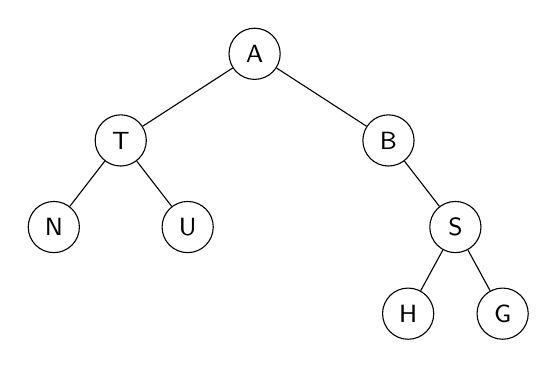
\begin{tikzpicture}[level distance=11mm,every node/.style={circle,draw,minimum size=6.5mm,inner sep=0pt,font=\small\sffamily},
  level 1/.style={sibling distance=34mm},level 2/.style={sibling distance=17mm},level 3/.style={sibling distance=12mm}]
\node {A} child {node {T} child {node {N}} child {node {U}}}
  child {node {B} child[missing] child {node {S} child {node {H}} child {node {G}}}};
\end{tikzpicture}
\end{center}
檢查：這棵樹的中序是 $N\,T\,U\,A\,B\,H\,S\,G$，後序是 $N\,U\,T\,H\,G\,S\,B\,A$，都和題目相同。 中序加上
後序（或前序）一定能唯一決定一棵二元樹（資結書定理~7.4 的做法），所以答案就是這一棵。 注意 $B$
只有右子節點，畫圖時要畫在右邊，否則中序會變成 $\ldots A\,H\,S\,G\,B$。
\end{pastsoln}
